%%%%%%%%%%%%%%%%%%%%%
%								%
%	APENDICES					%
%								%
%%%%%%%%%%%%%%%%%%%%%

\appendix
\newpage
\chapter{Apendice A}
\label{Apendice A}
Acá van los apéndices, aprovechando...

Nota: los archivos memoria.algo (con "algo" distinto de "tex") se generan automáticamente al compilar, algunos errores con la bibliografía pueden solucionarse borrándolos y re-compilando.

\chapter{Teoria de Grafos}\label{ap:apendice_graph_theory}
inicio de mi grafo \cite{book_introduction_graph_theory}
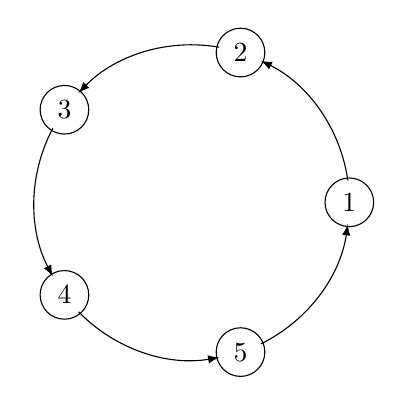
\begin{tikzpicture}

\def \n {5}
\def \radius {2cm}
\def \margin {8} % margin in angles, depends on the radius

\foreach \s in {1,...,\n}
{
test
  \node[draw, circle] at ({360/\n * (\s - 1)}:\radius) {$\s$};
  \draw[->, >=latex] ({360/\n * (\s - 1)+\margin}:\radius) 
    arc ({360/\n * (\s - 1)+\margin}:{360/\n * (\s)-\margin}:\radius);
}
\end{tikzpicture}

Final de mi grafo

\chapter{Catalog management handled with relational databases}\label{ap:apendice_ecommerce_catalog_relational}

\begin{figure}[h!]
	\centering
	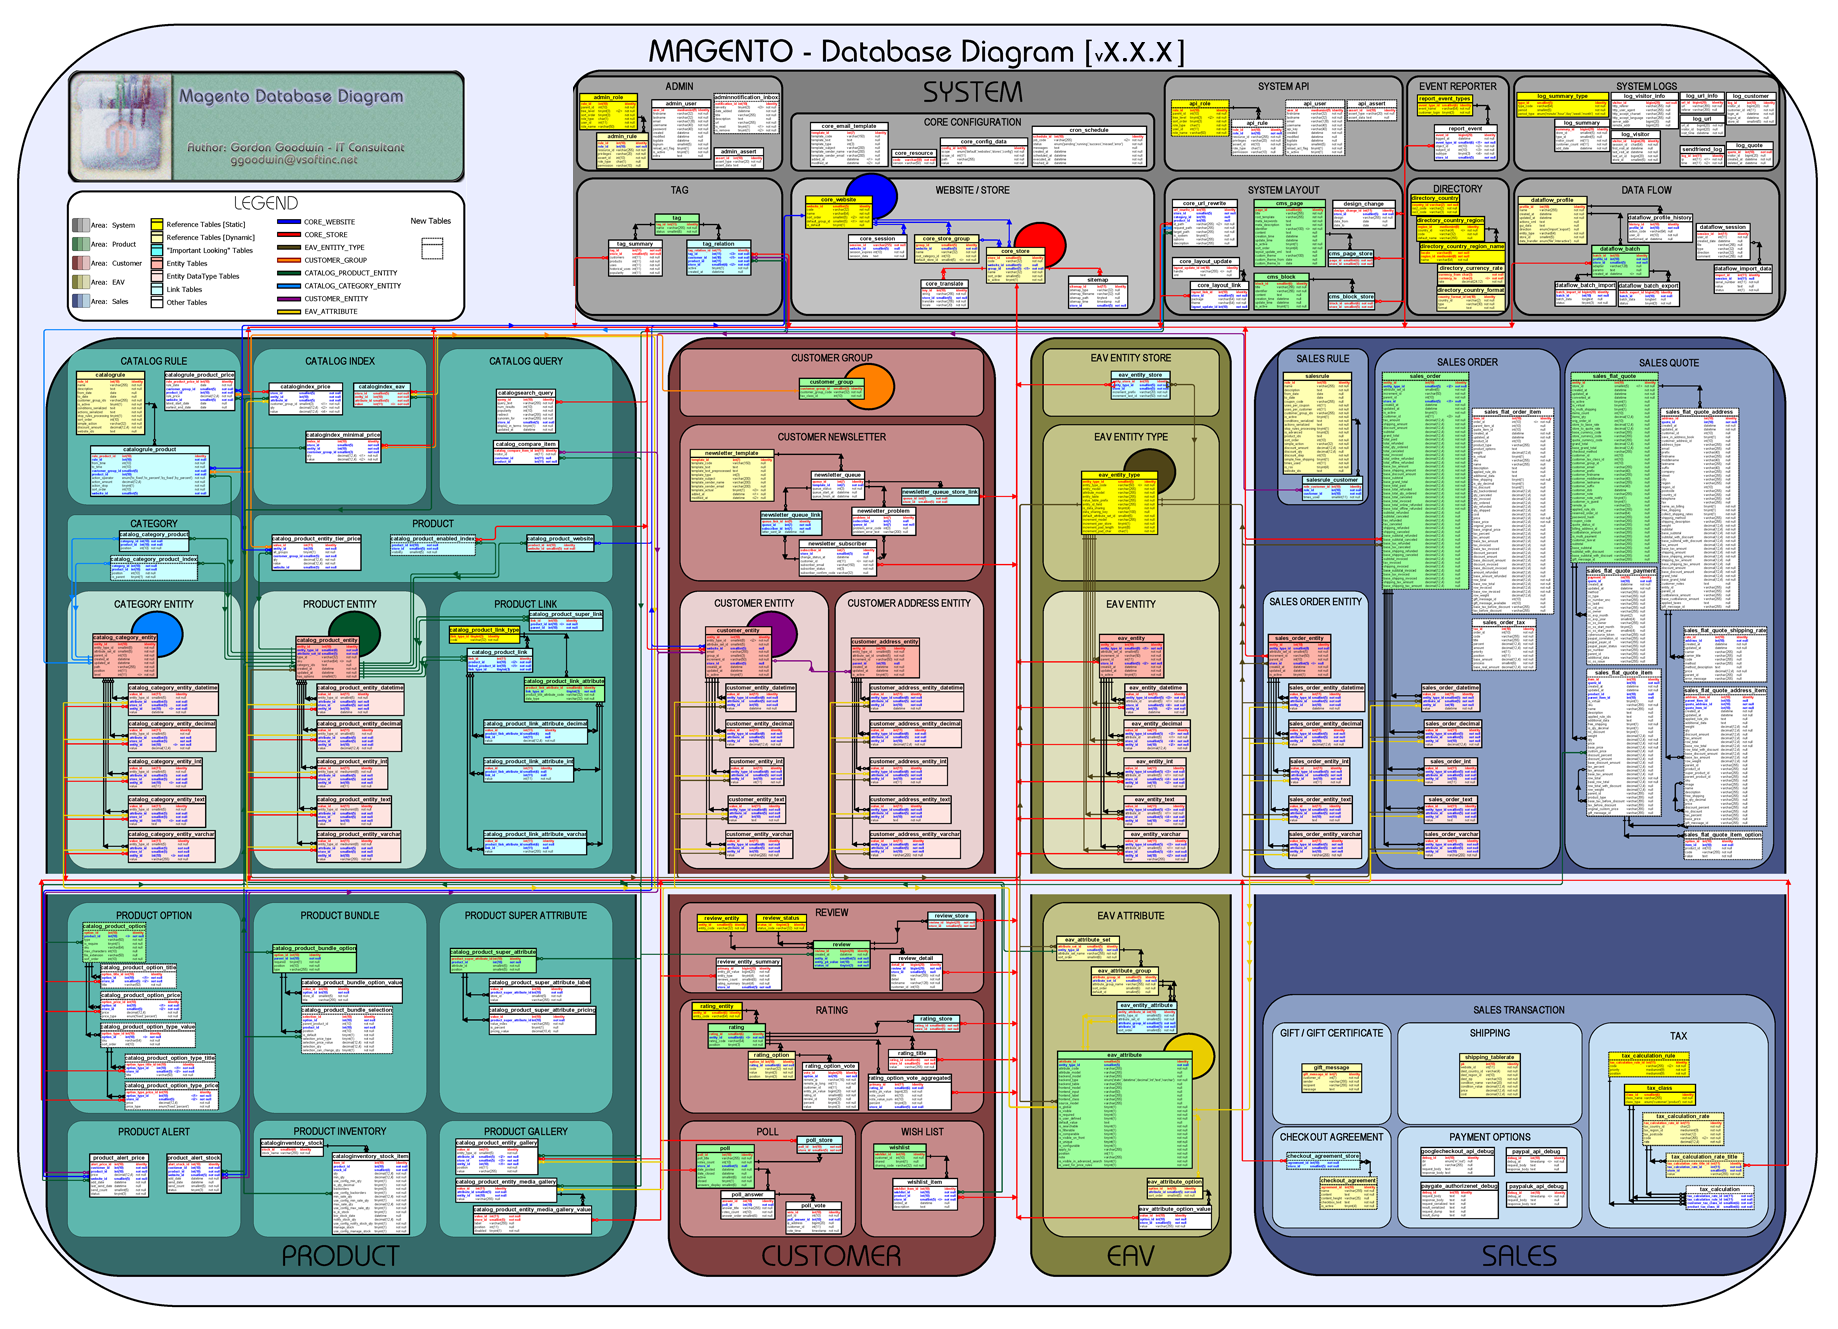
\includegraphics[width=0.8\textwidth]{figuras/apendice/magento_sample_database_diagram.png}
	\caption{schemas of Magento e-commerce framework.}
	\label{ap:figure:catalog_magento}
\end{figure}

\begin{figure}[h!]
	\centering
	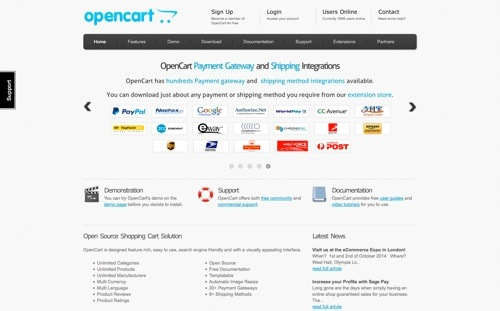
\includegraphics[width=0.5\textwidth]{figuras/apendice/openCartWebsite.jpg}
	\caption{schemas of the Apache's OfBiz.}
	\label{ap:figure:catalog_ofbiz}
\end{figure}

\chapter{¿Qué es Hadoop? \cite{online_hadoop_description}}\label{ap:apendice_hadoop_description}
Apache™ Hadoop® es un proyecto software \textit{open source} que permite el procesamiento distribuido de gran cantidad de datos a través de \textit{clusters} de servidores. Esta diseñado para \textit{scale up} desde un único servidor a miles de machinas, con un muy alto grado de tolerancia al fallo. En lugar de confiar en \textit{high-end hardware}, la flexibilidad de estos \textit{clusters} proviene de la habilidad del software en detectar y manejar fallos en la \textit{application layer}.

\subsubsection*{High-level architecture} 
Apache Hadoop tiene dos pilares:

\begin{itemize}
	\item \gloss{hadoop_yarn} asigna CPU, memoria y almacenamiento para las aplicaciones corriendo en Hadoop clústers. La primera generación de Hadoop podia solo correr aplicaciones \gloss{hadoop_mapreduce}. \gloss{hadoop_yarn} permite que otros entornos de aplicaciones (como SPARK) para ejecutarse en Hadoop, lo que abre un mundo de posibilidades.
	
	\item \gloss{hadoop_hdfs} es un sistema de archivos que se extiende por todos los nodos en su clúster Hadoop para almacenamiento de datos. Se conecta entre si a los sistemas de archivos en muchos nodos locales para convertirlos en un sistema de archivos grandes.
\end{itemize}

Hadoop se complementa con un ecosistema de proyectos de Apache, como Pig\cite{online_ibm_meaning_pig}, Hive\cite{online_ibm_meaning_hive} y Zookeeper\cite{online_ibm_meaning_zookeeper}, para extender el valor de Hadoop y mejorar su usabilidad.


\subsubsection*{Entonces, ¿Cuál es el problema?}

Hadoop cambia la economía y la dinámica de la computación a gran escala. Su impacto puede reducirse a cuatro características sobresalientes.

Hadoop permite una solución de computación que es:

\begin{itemize}
	\item \textbf{\textit{Scalable}}- Nuevos nodos pueden ser agregados según sean necesarios, y agregados sin la necesidad de cambiar el formato de los datos, como los datos son cargados, como los \textit{jobs} son escritos, o las aplicaciones en la parte superior.
	
	\item \textbf{\textit{Cost effective}}- Hadoop trae computación paralela masiva a las maquinas de los servidores. El resultado es una considerable disminución en los costos por \textit{terabyte} de almacenamiento. lo cual hace asequible para modelar todos sus datos.
	
	\item \textbf{\textit{Flexible}}- Hadoop no tiene esquema, y puede absorber cualquier tipo de datos, estructurados o no, desde cualquier numero de fuentes. Los datos de múltiples fuentes pueden ser unidos y se agregan arbitrariamente para permitir análisis que ningún otro sistema puede proporcionar.
	
	\item \textbf{\textit{Fault tolerant}}- Cuando se pierde un nodo, el sistema redirige el trabajo a otra ubicación de los datos y seguir con el procesamiento sin perder el ritmo.
\end{itemize}




		